\section{Operational Carbon Footprint Analysis}
Operation Carbon Footprint is the most important metric for the goal of our observation, since it is the result of combining energy usage (related to power consumption) and carbon intensity. \\
For this reason we will see a combination of the observations we did related both to power and CI, and our final suggestions will be a cross-reference of the previous data.

\vspace{-15pt}

\begin{figure}[H]
\centering
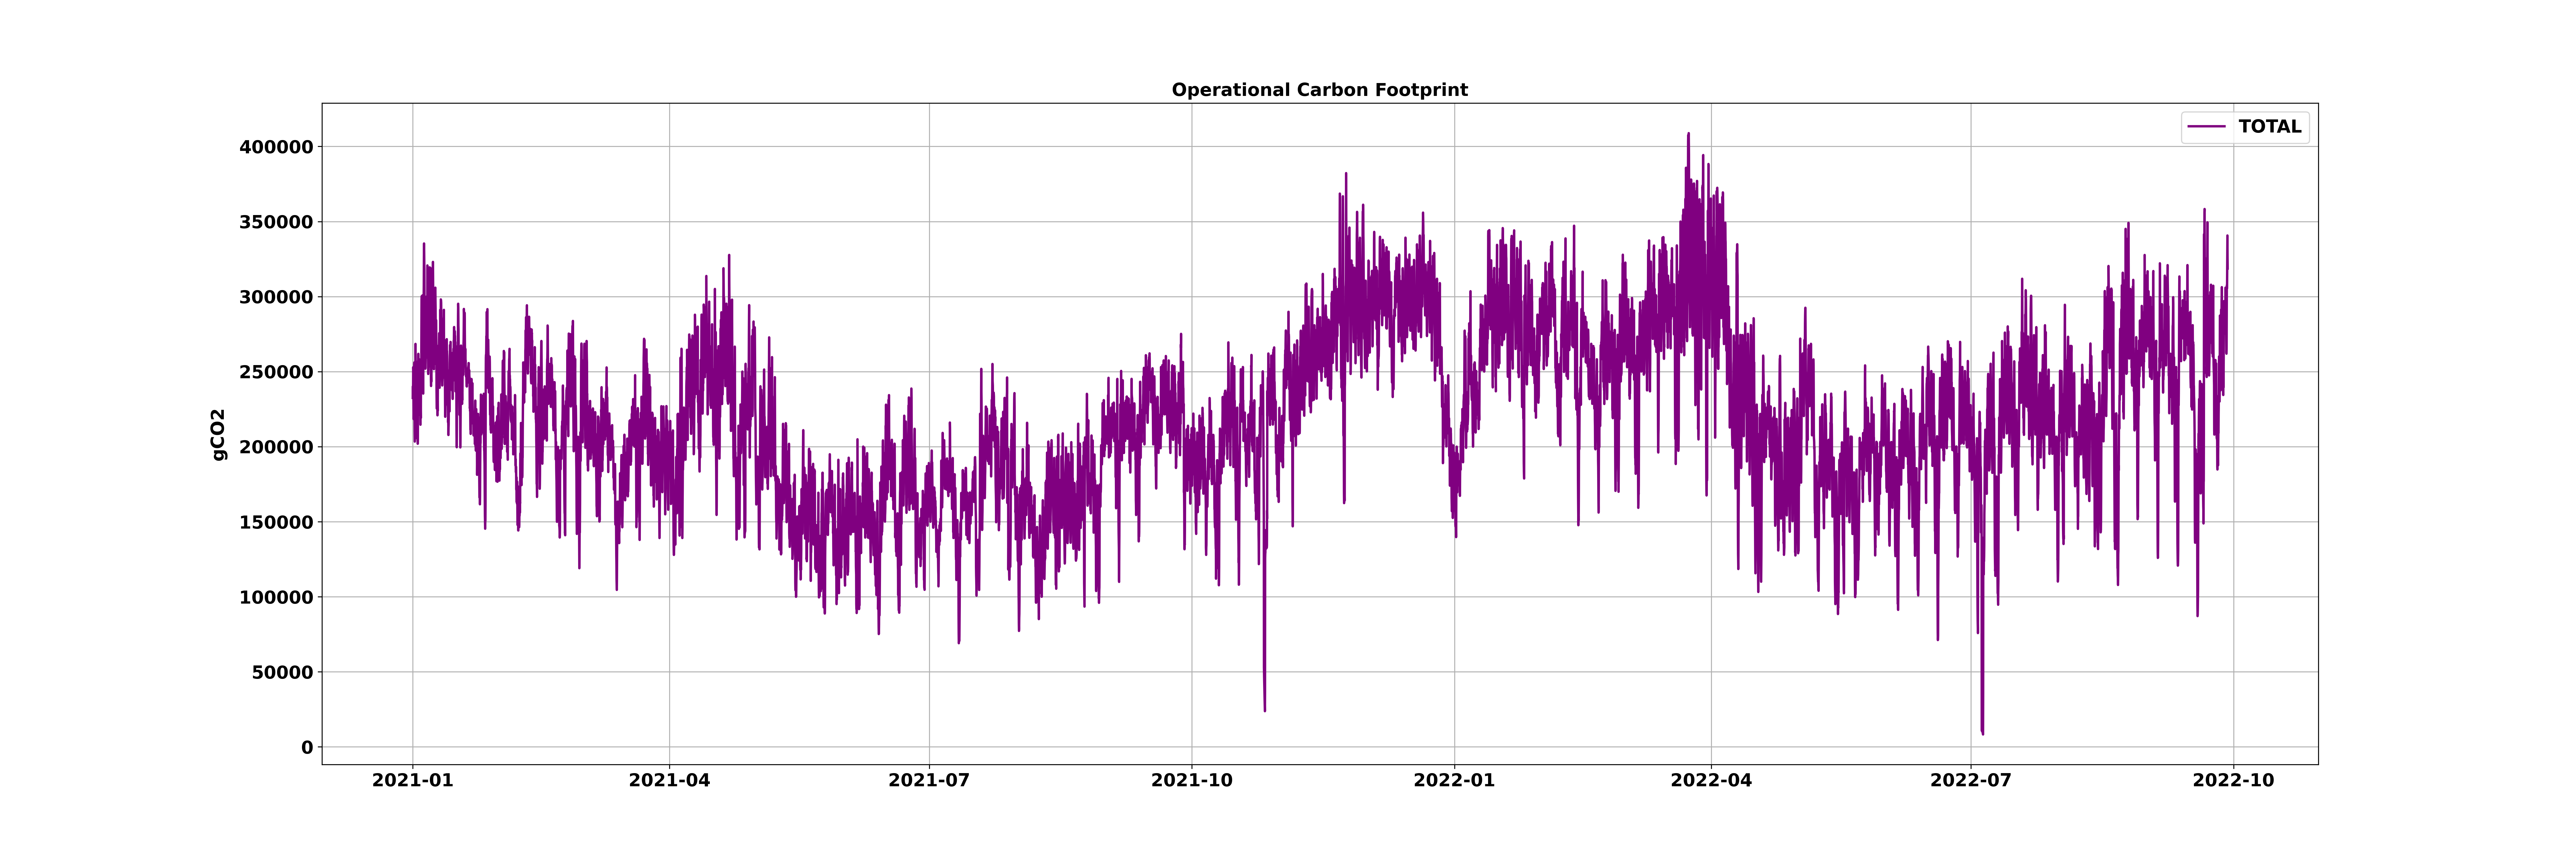
\includegraphics[width=1\textwidth]{../../PLOTS/Cop_total.png}
\captionsetup{skip=-10pt}
\caption{Cop total value (sum of all nodes in the server)}
\label{fig:Cop_total}
\end{figure}

\begin{center}
\setstretch{0.9}
count     15263.000000 \\
mean     220186.340067 \\
std       54400.325364 \\
min        8292.258962 \\
25\%      181522.725893 \\
50\%      218140.616056 \\
75\%      258846.427357 \\
max      408868.699240   
\end{center}

\subsection{Cop r206n01 STL}

\vspace{-10pt}

\begin{figure}[H]
\centering
\includegraphics[width=1\textwidth]{../../PLOTS/Cop_stl.png}
%\captionsetup{skip=-10pt}
\caption{Cop r206n01 STL}
\label{fig:Cop_r206n01_stl}
\end{figure}

\subsection{Cop analysis using Meta's Prophet}
As before, Prophet allows to better visualize the seasonality of our distribution: \\
in general the carbon footprint follows very much the carbon intensity distribution, showing the higher impact it has on the final pollution factor;
looking at the week level plot, we clearly see a big lowering in equivalent CO2 production during sunday, while the same happens every day close to noon (same observations we did on the CI). 
At season and month level we confirm that the footprint lowers during summer.

\vspace{-10pt}

\begin{figure}[H]
\centering
\includegraphics[width=1\textwidth]{../../PLOTS/Cop_prophet.png}
%\captionsetup{skip=-10pt}
\caption{Cop trends}
\label{fig:Cop_prophet}
\end{figure}